%Praesentationsmodus
\documentclass[t,aspectratio=169,divpsnames]{beamer}
%Die Beameroption aspectratio legt das verwendete Seitenverhaeltnis fest
%aspectratio=169	16:9 Seitenverhaeltnis
%aspectratio=1610	16:10 Seitenverhaeltnis
%aspectratio=43		4:3 Seitenverhaeltnis
%Die Beameroption envcountsect nummeriert Umgebungen wie theorem pro section durch.
%Die Beameroption divpsnames wird an das xcolor Paket durchgereicht.

%Handout-Generierung mit Foliennotizen (statt obiger Zeile für den Präsentationsmodus verwenden)
%\documentclass[t,handout,aspectratio=169]{beamer}
%\setbeameroption{show notes}

\usepackage[utf8]{inputenc}

% Deutsch
%\usepackage[ngerman]{babel} 
%\usepackage{bibgerm}

% Englisch
\usepackage[english]{babel}

\mode<presentation>
{
\usetheme{HochschuleTrier}
\setbeamercovered{transparent}
}

%\usepackage{mathptmx}
%\usepackage[scaled=0.9]{helvet}
\usepackage{helvet}
\usepackage{courier}
%\usepackage{ae}

\usepackage{hyperref}
\usepackage{tikz}
\usepackage{amsmath}
\usepackage{amsfonts}

\logo{
\includegraphics[height=20.5mm]{UniKonstanz_Logo_Optimum.pdf}}

\usetikzlibrary{calc,positioning}

\usefonttheme[onlymath]{serif}

\usepackage{listings}
\usepackage{tikz}
\usepackage{lipsum}
\usepackage{listings}
\usepackage{xcolor}
\usepackage{siunitx}

\definecolor{codegreen}{rgb}{0,0.6,0}
\definecolor{codegray}{rgb}{0.5,0.5,0.5}
\definecolor{codepurple}{rgb}{0.58,0,0.82}
\definecolor{backcolour}{rgb}{0.95,0.95,0.92}

\long\def\/*#1*/{}

\lstset
{
	basicstyle=\ttfamily, 
	keywordstyle=\color{blue}\bfseries\ttfamily,
	identifierstyle=\ttfamily, 
	stringstyle=\ttfamily,
	commentstyle=\color{ForestGreen},
	showstringspaces=false,
	framexleftmargin=7mm, 
	breaklines=true,
	tabsize=3,
	showtabs=false,
	frame=single, 
	rulesepcolor=\color{blue},
	numbers=left,
	linewidth=146mm,
	xleftmargin=8mm,
	language={C++},
}
% Stil des Literaturverzeichnisses
\bibliographystyle{geralpha}
%\bibliographystyle{alpha}
%\bibliographystyle{abstract}

%Bitte ausfuellen:
\title{VR / AR}
\subtitle{Slides for the Course}
\author{D. Rumscheid, F. Kunze, J. de Boer, F. Kalchschmid}
\institute{Universität Konstanz}
\date{28.10.2023}
\subject{Immersive Analytics with Applications in the Life Sciences}

%Inhaltsverzeichnisses bis auf subsubsection-Ebene:
%\setcounter{tocdepth}{3}

%Aktivieren, um am Anfang jeder Section ein Inhaltsverzeichnis zur Section anzuzeigen
%\AtBeginSection[]
%{
%\begin{frame}<beamer>
%\frametitle{Agenda}
%\tableofcontents[currentsection,hideothersubsections,sectionstyle=show/hide,subsubsectionstyle=show/show]
%\end{frame}
%}

%Aktivieren, um alles Schritt-fuer-Schritt einzublenden
%\beamerdefaultoverlayspecification{<+->}

\begin{document}

\begin{frame}
\titlepage
\end{frame}

%\begin{frame}
%\frametitle{Agenda}
%\tableofcontents
%\tableofcontents[hideallsubsections] % Subsections ausblenden
%\tableofcontents[pausesections] %Sections Schritt-fuer-Schritt einblenden
\end{frame}

\section{Milestones}
\begin{frame}{Milestones}{Timeline of Development}
\begin{columns}[T]

\begin{column}[T]{0.27\textwidth}
\textbf{Milestone 1}
\begin{itemize}
\item Vertical Slice
\item Critical Components
    \begin{itemize}
        \item Interactable Module
     ´  \item Display Module
        \item Tasks    
        \item Game Manager 
    \end{itemize}
\item Asynchronous Player Interaction
\end{itemize}
\end{column}
\begin{column}{0.27\textwidth}
\textbf{Milestone 2}
\begin{itemize}
    \item Implement new creative Interaction Ideas based on the base system.
    \item Horizontal Growth of the Game
    \item Sketches of each Interaction \cite{Buxton.2012}
\end{itemize}
\end{column}
\begin{column}{0.20\textwidth}
\textbf{Milestone 3}
	\begin{itemize}
	    \item Adding visual components to make the tasks more immersive.
	\end{itemize}
\end{column}
\begin{column}{0.35\textwidth}
\textbf{Milestone 4}
\begin{itemize}
    \item Adding more complex riddles and interactions
    \item Interdependent Tasks built upon existing components
    \item Visual- and Usability-Polishing    
\end{itemize}
\textbf{\textsc{Optional:} Milestone 5}
\begin{itemize}
    \item Adding 2nd player to VR with his own interactions and tasks.  
\end{itemize}
\end{column}
\end{columns}
\end{frame}
\begin{frame}{Milestones}
\textbf{Interaction Concepts} 
\begin{itemize}
    \item All interactions work with the VR-Controllers and Motion Tracking of Quest 2.
\end{itemize}
\textbf{Why does the Project Idea Work in VR?}
\begin{itemize}
    \item  The riddles require you to move in 3D space in a room.
    \item The interactions replicate real physical world interaction in a virtual context.
    \item Players perspectives are different (VR / PDF Manual), communication required.
\end{itemize}
\textbf{How do you deal with common issues in VR environments?} 
\begin{itemize}
    \item Little peripheral movement (only things relevant to the riddles)
    \item One local setting with a limited playing area. Submarine as closed environment.
    \item Cartoon visuals: Helps performance and supports immersion.
    \item Each gameplay module is designed to respect the field of view.
\end{itemize}
\end{frame}
\begin{frame}{Milestones}{Project Timeline \& Modules}
    \begin{figure}
    \vspace{-0.1cm}
	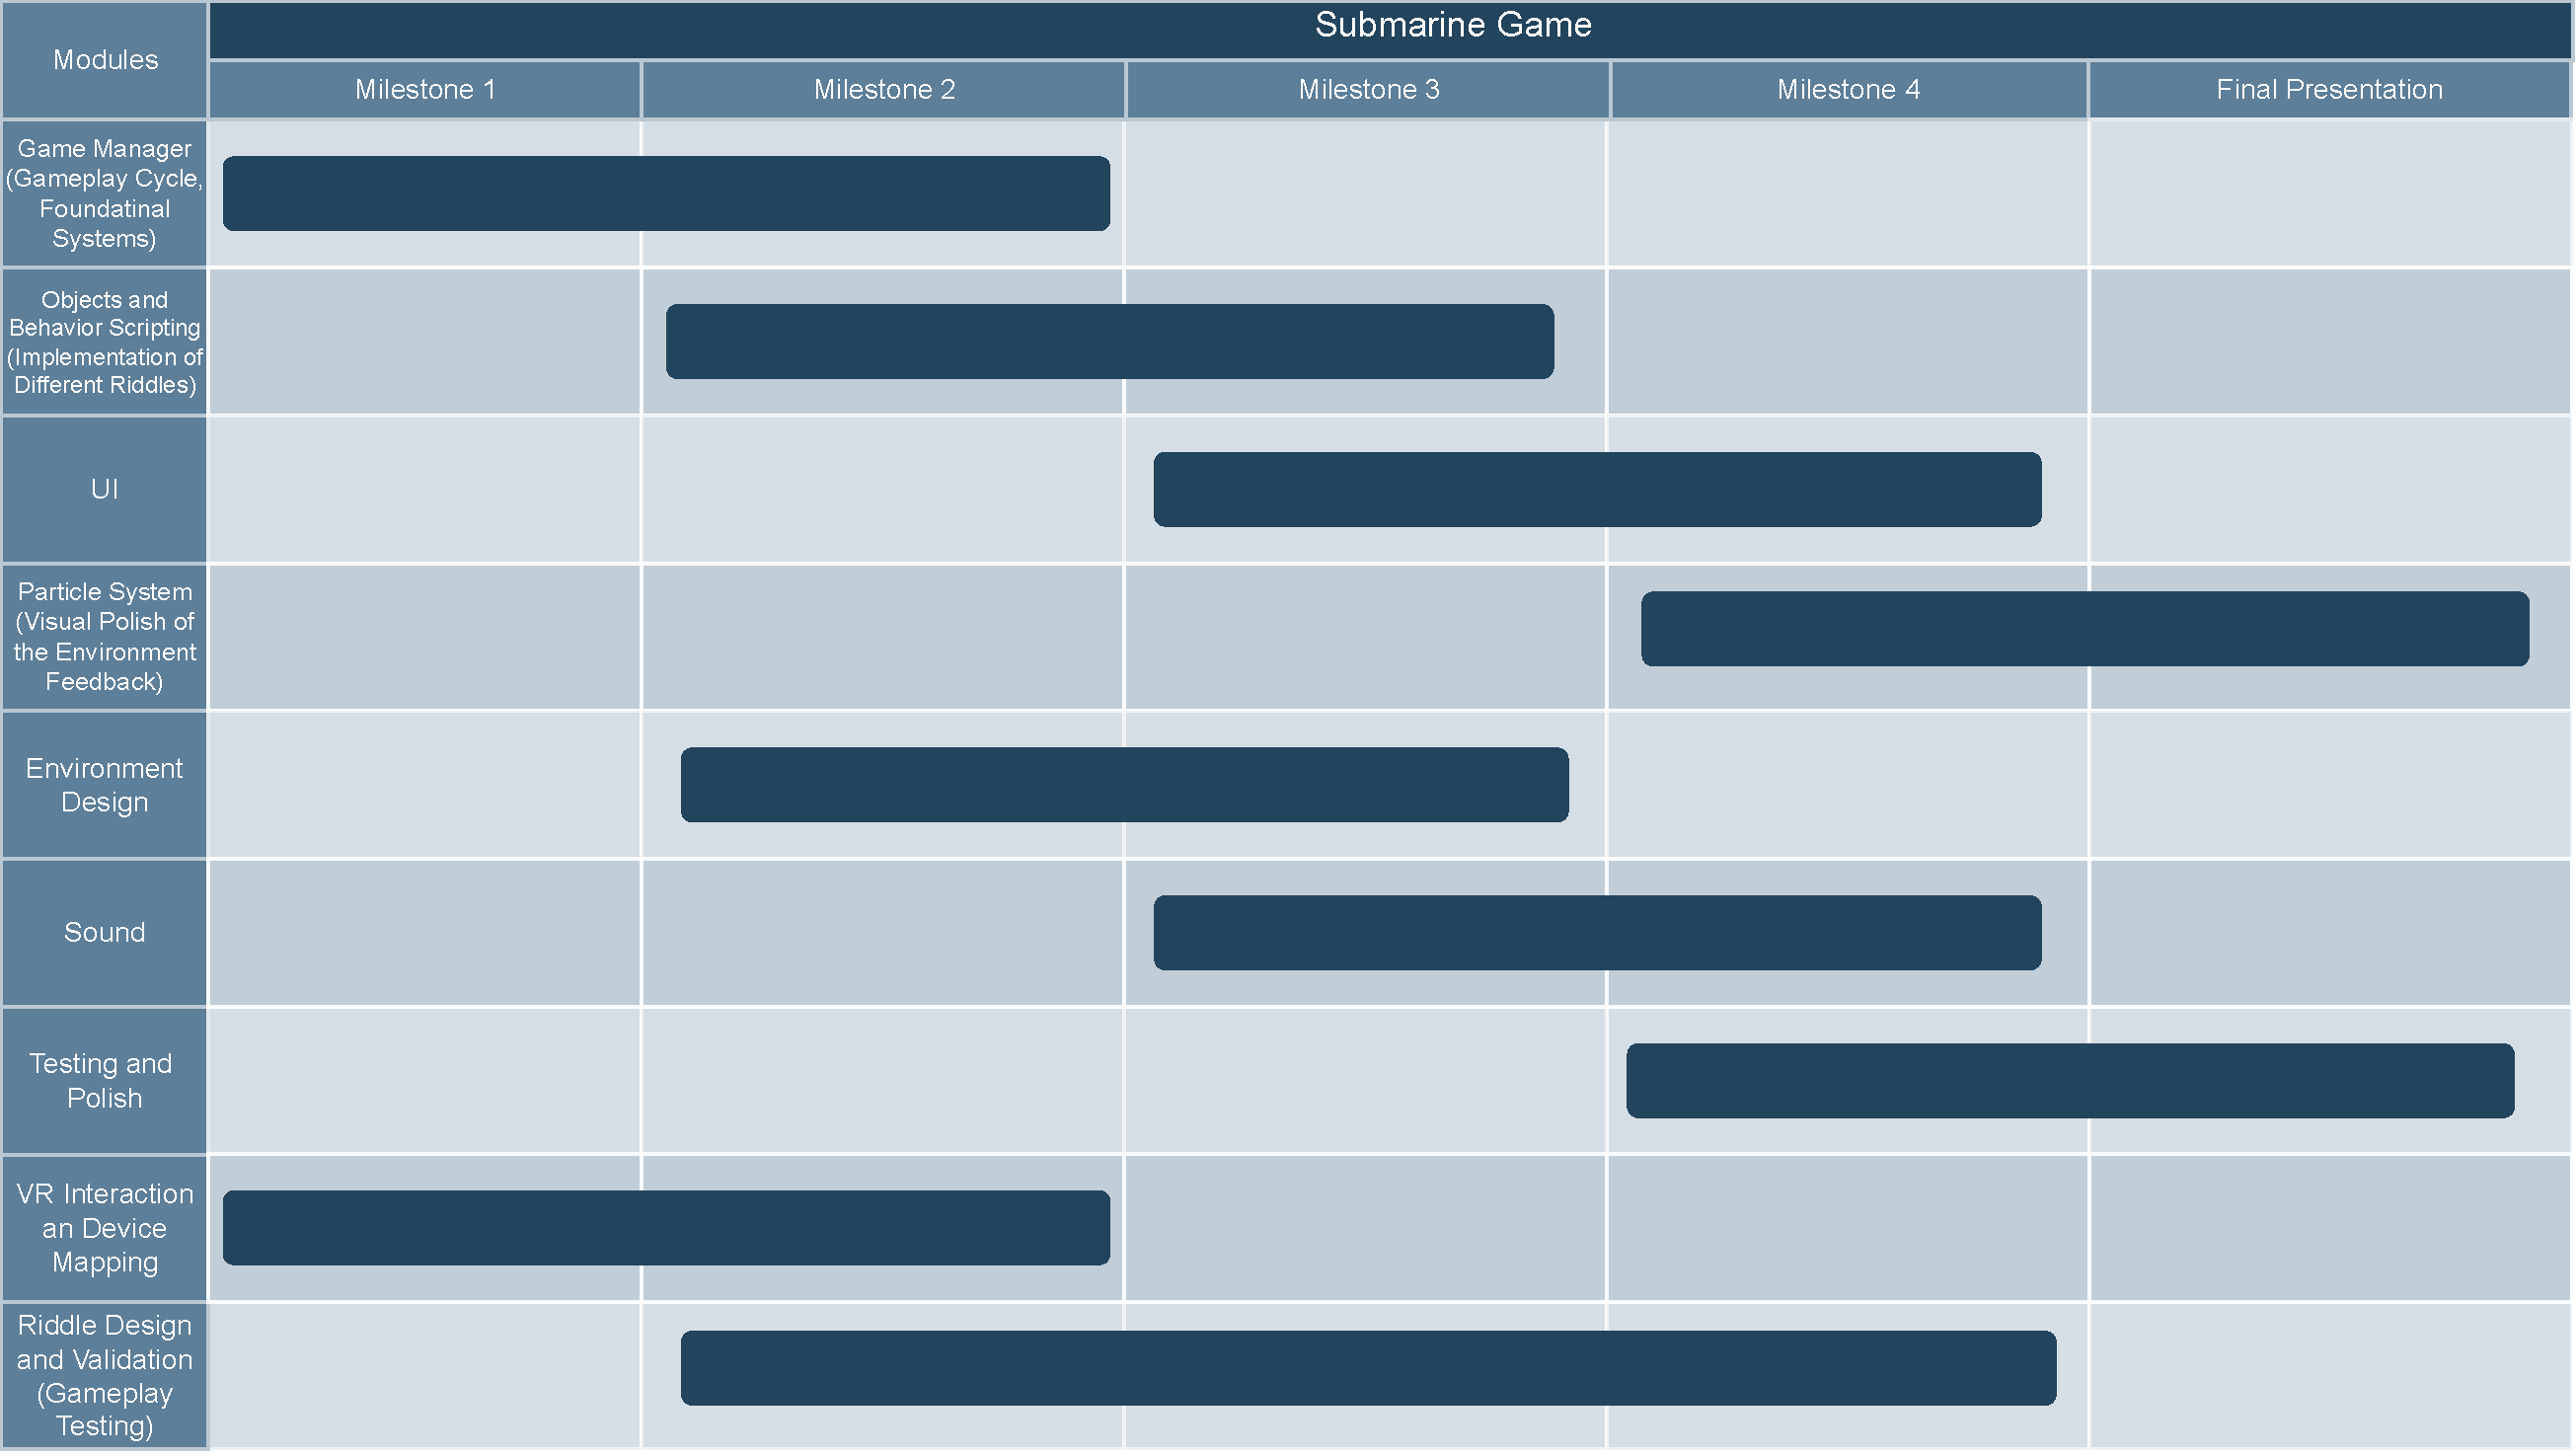
\includegraphics[width=11cm]{images/Timeline_VR-AR.pdf}
	
\end{figure}
\end{frame}
\subsection{Milestone 1}
\begin{frame}{Milestone 1}{Needed Interactions \& Systems}
    \begin{figure}
    \vspace{-0.1cm}
	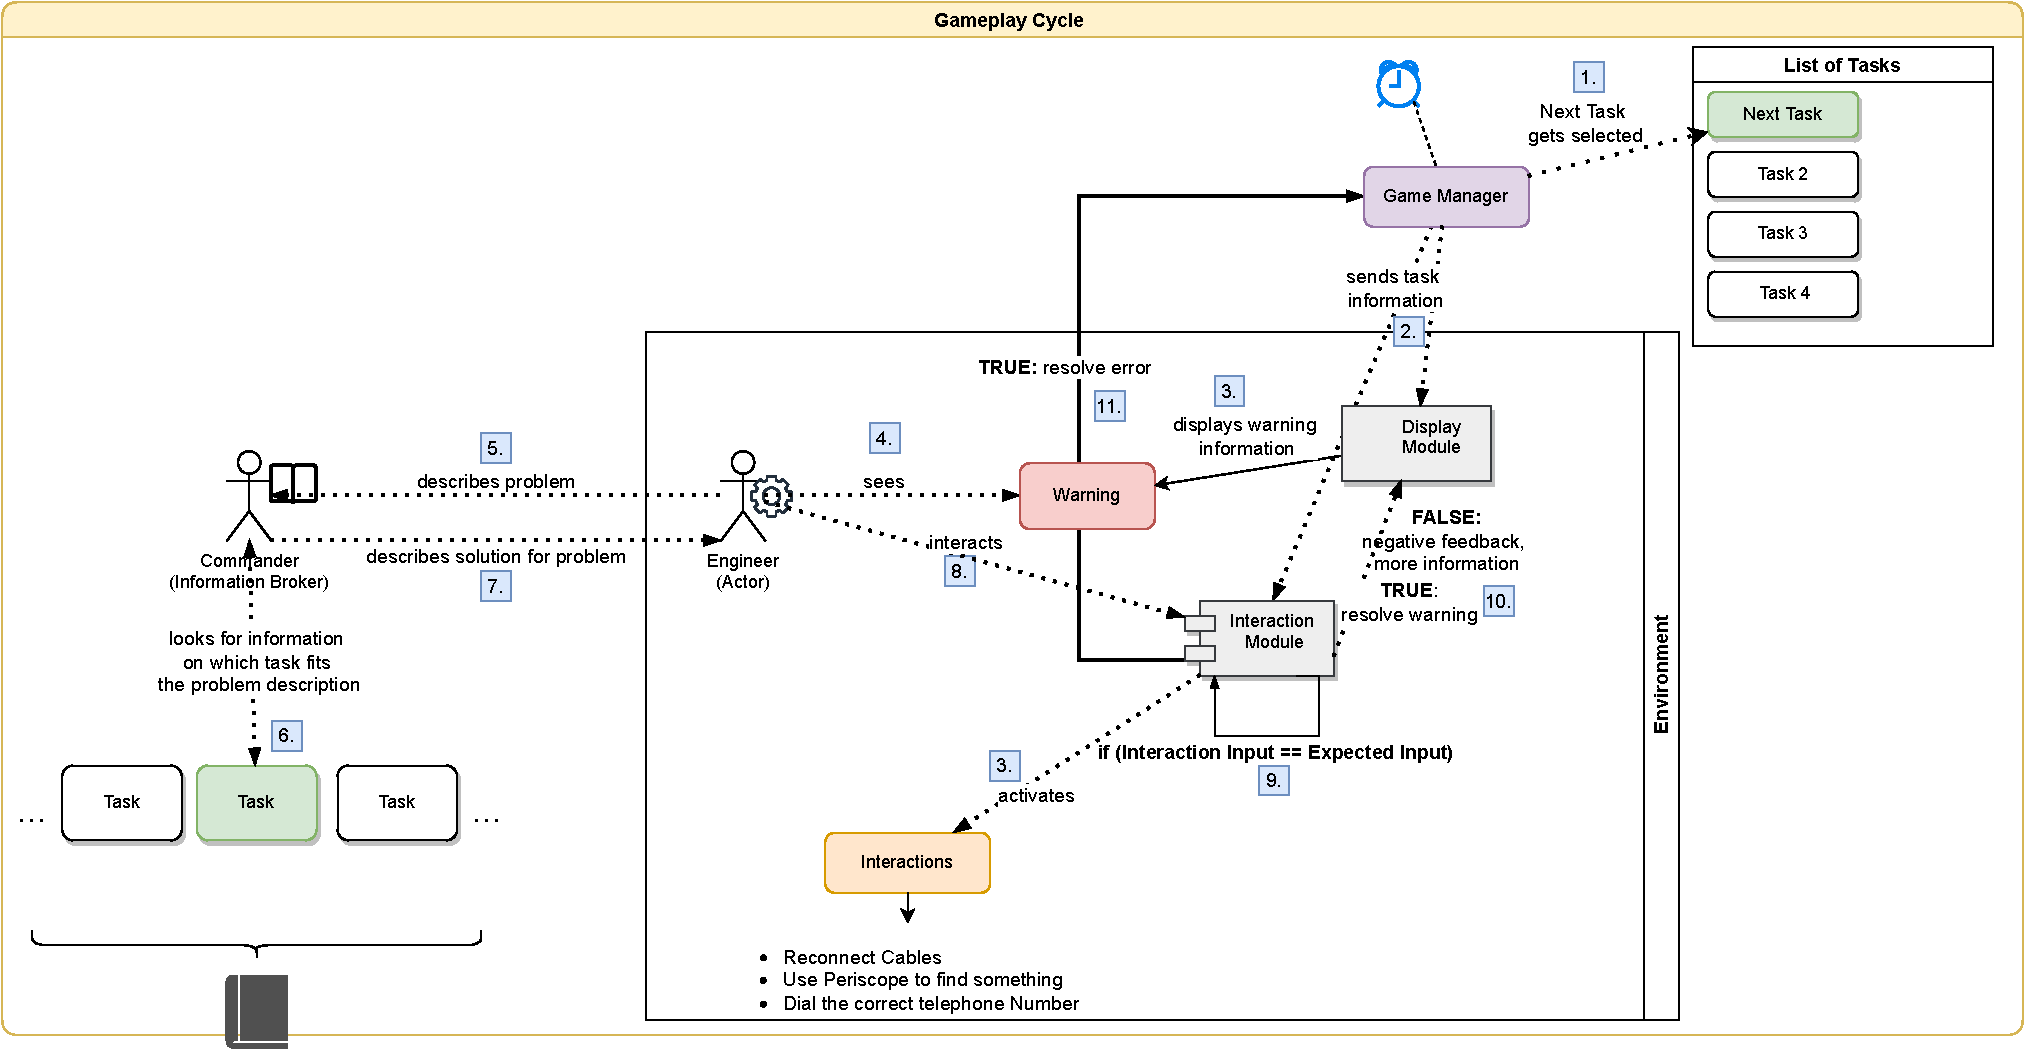
\includegraphics[width=12.5cm]{images/gameplay_cycle.pdf}
	
\end{figure}
\end{frame}

\begin{frame}{Milestone 1}{Very Rough First System Design}
    \begin{figure}
	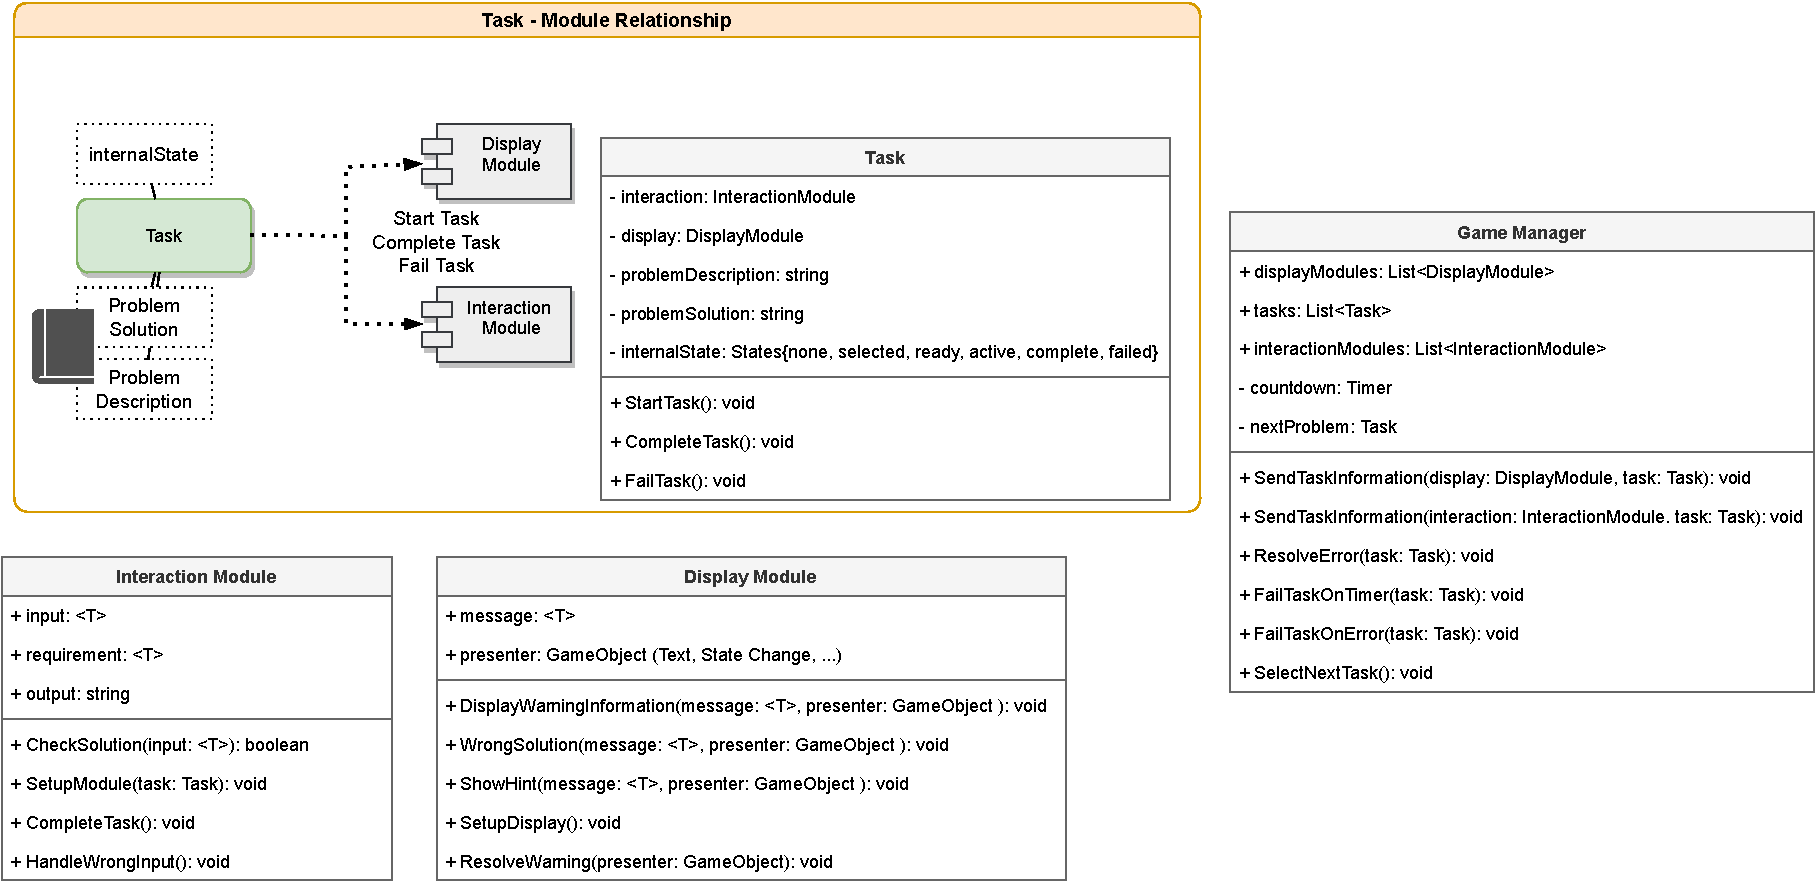
\includegraphics[width=12.5cm]{images/system_architecture.pdf}
     \vspace{-1.0cm}
\end{figure}
\end{frame}
\section*{End}
%\begin{frame}
%	\begin{center}
%		\huge{Thank you for your attention.}
%	\end{center}
%	\begin{center}
%		\Huge{Questions?}
%	\end{center}
%\end{frame}

\begin{frame}[allowframebreaks]{\bibname}
\bibliography{literatur}     %BibTeX-Datei literatur.bib
\end{frame}


\end{document}
